\documentclass[12pt,a4paper]{article}

\usepackage{amsmath,amssymb}
\usepackage{graphicx}
\usepackage{float}
\usepackage{booktabs}
\usepackage{geometry}
\usepackage{setspace}
\usepackage{caption}
\usepackage{subcaption}
\usepackage{hyperref}

\usepackage{listings}
\usepackage{xcolor}

\lstdefinestyle{matlab}{
    language=Matlab,
    basicstyle=\ttfamily\scriptsize,
    keywordstyle=\color{blue},
    commentstyle=\color{green!50!black},
    stringstyle=\color{red},
    numbers=left,
    numberstyle=\tiny,
    stepnumber=1,
    numbersep=10pt,
    frame=single,
    breaklines=true,
    tabsize=2,
    showstringspaces=false
}

\lstdefinestyle{verilog}{
    language=Verilog,
    basicstyle=\ttfamily\scriptsize,
    keywordstyle=\color{blue},
    commentstyle=\color{green!50!black},
    stringstyle=\color{red},
    numbers=left,
    numberstyle=\tiny,
    stepnumber=1,
    numbersep=10pt,
    frame=single,
    breaklines=true,
    tabsize=2,
    showstringspaces=false
}

\lstdefinestyle{Python}{
    language=Python,
    basicstyle=\ttfamily\scriptsize,
    keywordstyle=\color{blue},
    commentstyle=\color{green!50!black},
    stringstyle=\color{red},
    numbers=left,
    numberstyle=\tiny,
    stepnumber=1,
    numbersep=10pt,
    frame=single,
    breaklines=true,
    tabsize=2,
    showstringspaces=false
}


\geometry{margin=1in}
\onehalfspacing

\title{\textbf{EE2801 - DSP LAB \\ EXPERIMENT-2} \\
Fixed-Point Arithmetic using Verilog}
\author{EE24BTECH11012 - BHAVANISANKAR G S}
\date{\today}

\begin{document}
\maketitle

\tableofcontents
\newpage

\section{Plots}

\begin{figure}[H]
    \centering
    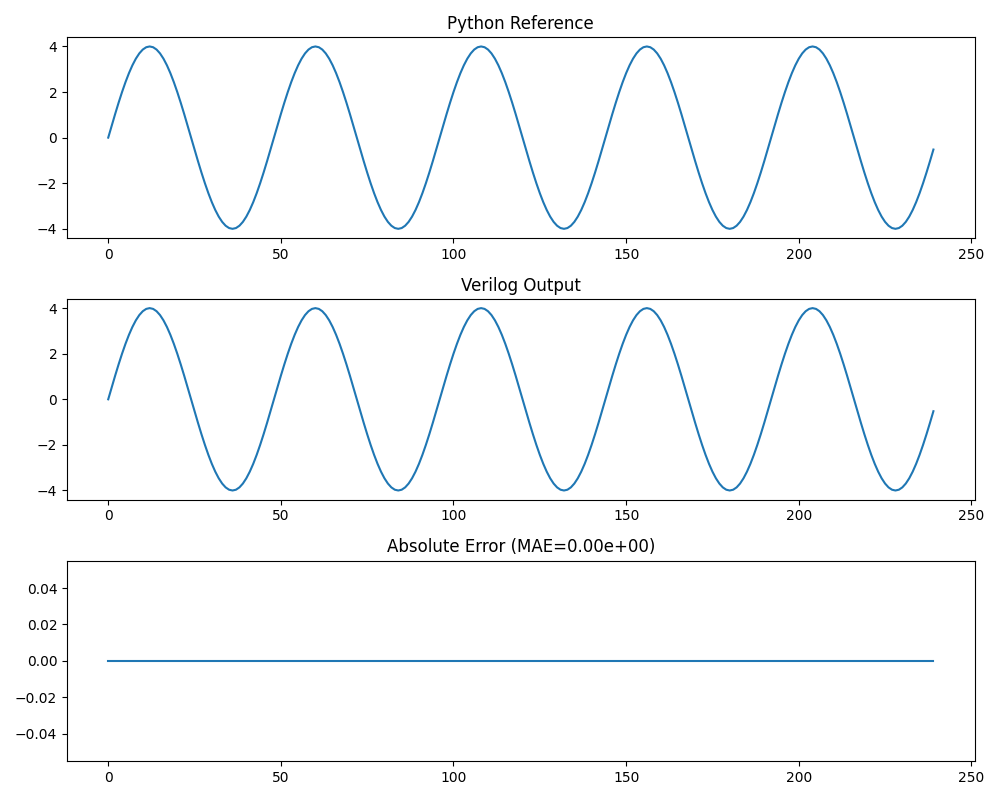
\includegraphics[width=0.8\linewidth]{figs/add.png}
    \caption{Addition results}
    \label{fig:placeholder}
\end{figure}

\begin{figure}[H]
    \centering
    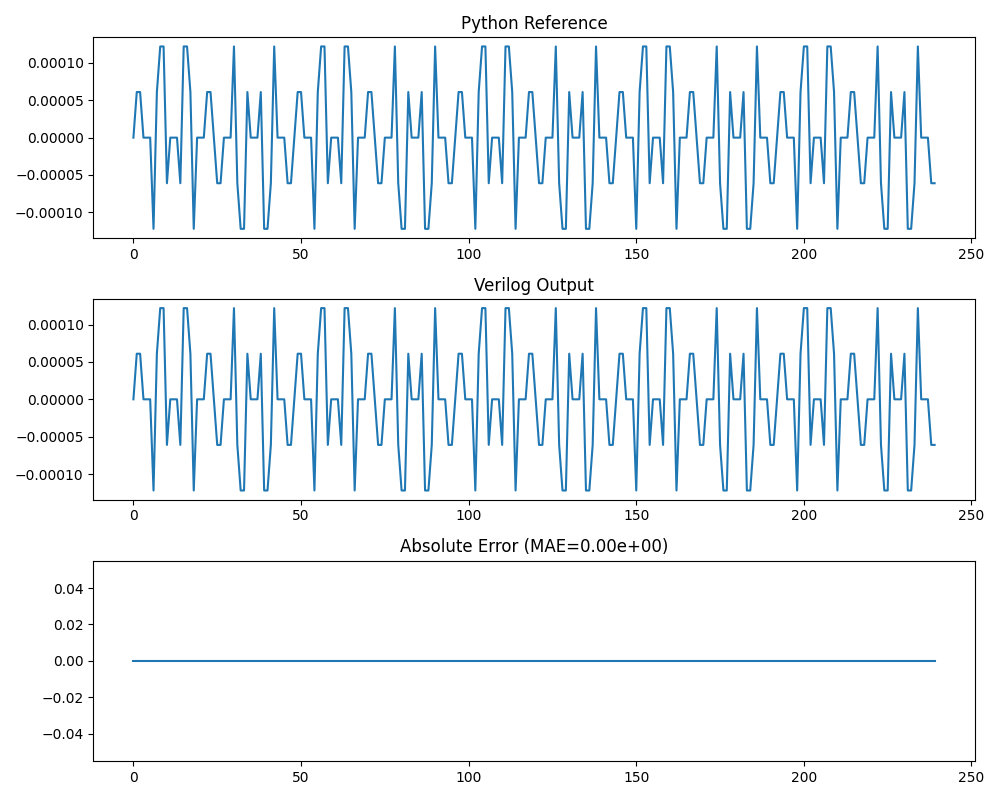
\includegraphics[width=0.8\linewidth]{figs/sub.png}
    \caption{Subtraction results}
    \label{fig:placeholder}
\end{figure}

\begin{figure}[H]
    \centering
    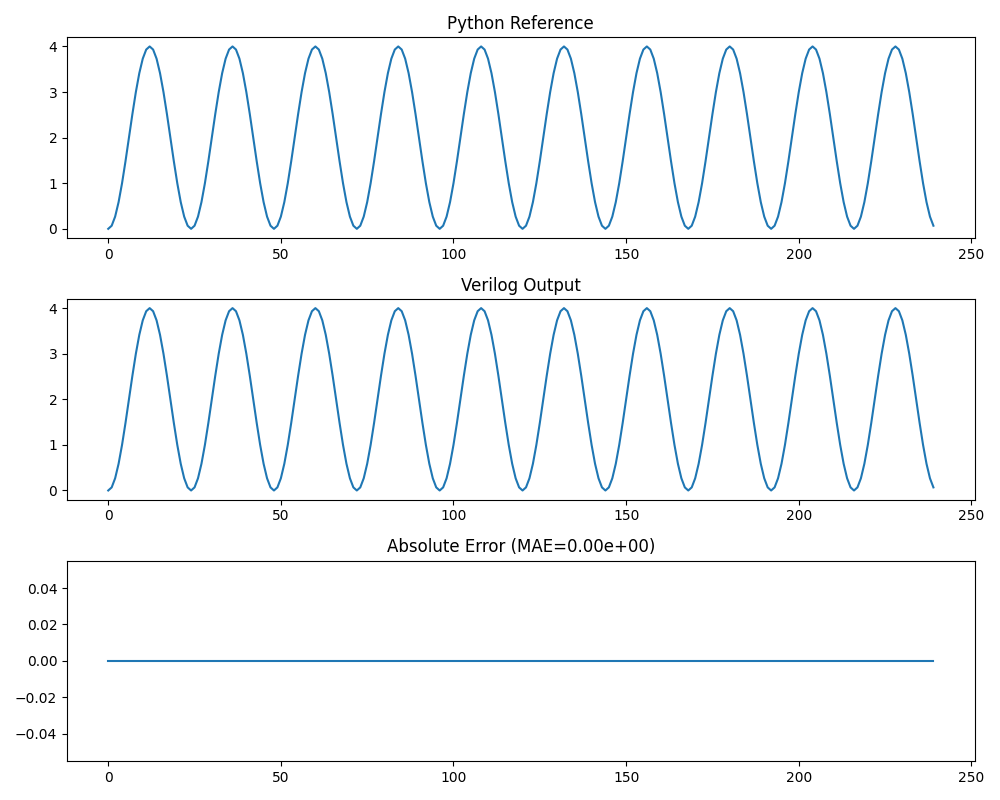
\includegraphics[width=0.8\linewidth]{figs/mul.png}
    \caption{Multiplication results in Q(10, 28) format}
    \label{fig:placeholder}
\end{figure}

\begin{figure}[H]
    \centering
    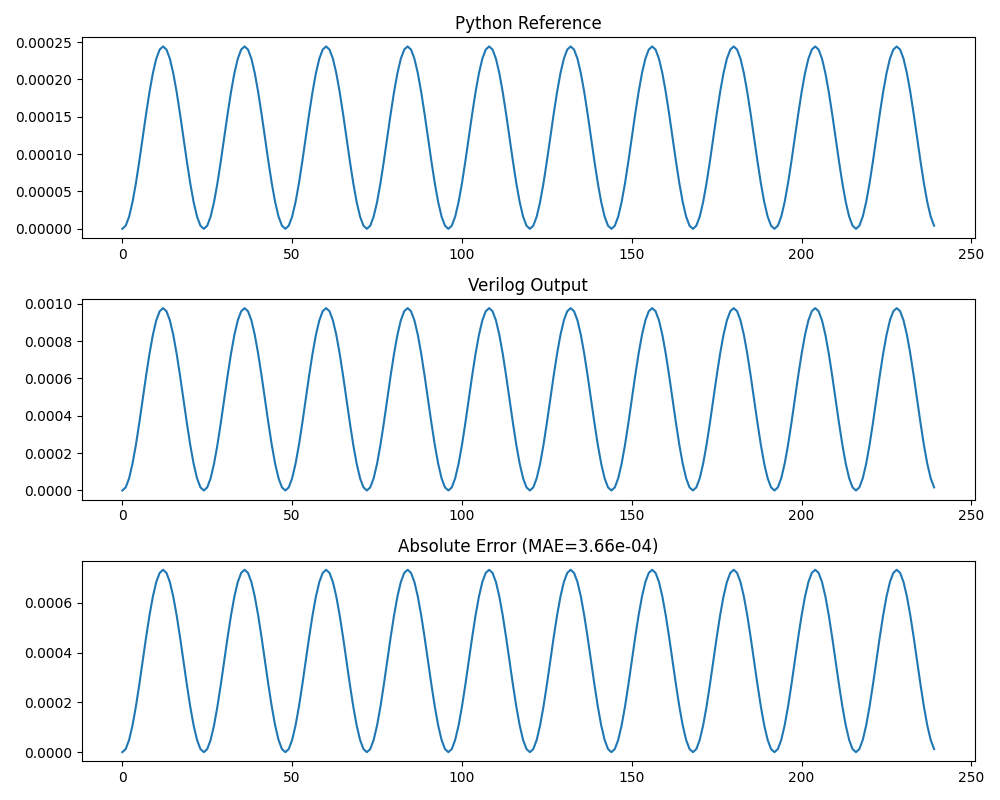
\includegraphics[width=0.8\linewidth]{figs/mul_eff.png}
    \caption{Multiplication results in Q(10, 14) format - Hardware Efficient}
    \label{fig:placeholder}
\end{figure}

\section{Observations}

\begin{figure}[H]
    \centering
    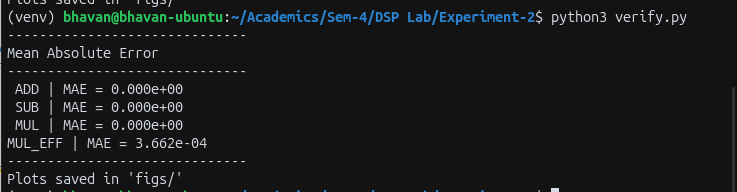
\includegraphics[width=\linewidth]{errors_analysis.png}
    \caption{Errors obtained comparing Python and Verilog outputs}
    \label{fig:placeholder}
\end{figure}
\begin{itemize}
    \item Fixed-point addition and subtraction operations produced outputs that exactly matched the Python floating-point reference model, resulting in zero mean absolute error (MAE).
    
    \item Subtraction of two signals derived from the same sinusoidal waveform resulted in a small-amplitude output, which is expected due to minor fixed-point quantization differences between operands.
    
    \item Full-precision fixed-point multiplication, retaining the complete fractional growth (Q(10,28)), showed zero numerical error when compared with the Python reference.
    
    \item A hardware-efficient multiplication approach (MUL\_EFF), obtained by right-shifting the full-precision product by $\text{FRAC}_{\max}$ bits to restore the original fractional width (Q(10,14)), introduced a small bounded quantization error.
    
    \item The measured mean absolute error for the MUL\_EFF operation was $3.662 \times 10^{-4}$, consistent with theoretical truncation error limits.
\end{itemize}

\section{Conclusions}

\begin{itemize}
    \item Fixed-point arithmetic can accurately replicate floating-point computations when proper Q-format alignment and scaling are applied.
    
    \item Full-precision multiplication ensures bit-exact accuracy but incurs increased hardware cost due to significant bit-width growth.
    
    \item Truncating the multiplier output to limit fractional precision introduces a predictable and bounded quantization error while substantially improving hardware efficiency.
    
    \item The MUL\_EFF approach provides an effective trade-off between numerical accuracy and FPGA resource utilization, making it suitable for real-time DSP applications.
    
    \item The close agreement between Python reference results and Verilog outputs validates the correctness and robustness of the fixed-point ALU implementation.
\end{itemize}

\section{Codes}

\begin{lstlisting}[style=matlab, caption={MATLAB code for Signal Generation}]
clc ;
close all ;
clear all ;

N = 240 ; % No of samples
f = 1e3 ;
fs = 10e3 ;
t = 0:1/fs:(5e-2 - 1/fs) ;

x = 2 * sin(2 * pi * f * t) ;
total_len = 17 ;
frac_len = 14 ;
fixed = fi(x, 1, total_len, frac_len) ;

filename = 'files/op1_bin.txt' ;
file = fopen(filename, 'w') ;

fprintf(file, "// %d %d\n", total_len - frac_len, frac_len) ;
for k = 1:length(x)
    fprintf(file, "%s\n", bin(fixed(k))) ;
end

fprintf('Data generated for Q(%d, %d) and written into the file %s\n', total_len-frac_len, frac_len, filename) ;
\end{lstlisting}

\begin{lstlisting}[style=verilog, caption={Verilog testbench module for printing values into a file}]
// W - Width of the fixed-point number
// FRAC - No of fractional bits
module align_frac #(
    parameter W_IN = 17,
    parameter W_OUT = 19,
    parameter FRAC_IN = 14,
    parameter FRAC_OUT = 14
) (
    input  signed [W_IN-1:0] in,
    output signed [W_OUT-1:0] out
);

wire signed [W_OUT-1:0] temp ;
assign temp = in ;

parameter SHIFT = FRAC_OUT - FRAC_IN ;
assign out = (SHIFT > 0) ? (temp << SHIFT) : ((SHIFT) ? (temp >>> (-SHIFT)) : temp) ;

endmodule

// Module to perform fixed-point addition
module fxp_add #(
    parameter WIDTH = 17
) (
    input  signed [WIDTH-1:0] a,
    input  signed [WIDTH-1:0] b,
    output signed [WIDTH-1:0] out
);
    
    assign out = a + b ;

endmodule

// Module to perform fixed-point subtraction
module fxp_sub #(
    parameter WIDTH = 17
) (
    input  signed [WIDTH-1:0] a,
    input  signed [WIDTH-1:0] b,
    output signed [WIDTH-1:0] out
);
    
    assign out = a - b ;

endmodule

// Module to perform fixed-point multiplication
module fxp_mul #(
    parameter WIDTH = 17
) (
    input  signed [WIDTH-1:0] a,
    input  signed [WIDTH-1:0] b,
    output signed [2*WIDTH-1:0] out
);

   assign out = a * b ;

endmodule

module fxp_alu #(
    parameter Q_IN1 = 3,
    parameter Q_IN2 = 5,
    parameter FRAC_IN1 = 14,
    parameter FRAC_IN2 = 12,
    parameter WIDTH = 19
) (
    input  signed [Q_IN1+FRAC_IN1-1:0] op1,
    input  signed [Q_IN2+FRAC_IN2-1:0] op2,
    output signed [WIDTH-1:0] op_add,
    output signed [WIDTH-1:0] op_sub,
    output signed [2*WIDTH-1:0] op_mul,
    output signed [Q_MAX+FRAC_MAX-1:0] mul_eff
);
    
    parameter Q_MAX = ( Q_IN1 > Q_IN2 ) ? Q_IN1 : Q_IN2 ;
    parameter FRAC_MAX = ( FRAC_IN1 > FRAC_IN2 ) ? FRAC_IN1 : FRAC_IN2 ;
    parameter W_ALIGNED = Q_MAX + FRAC_MAX ;
    parameter W_IN = Q_IN1 + FRAC_IN1 ;

    wire signed [W_ALIGNED-1:0] op1_aligned, op2_aligned ;
    // wire signed [Q_MAX_FRAC_MAX-1:0] mul_eff ;

    align_frac #(W_IN, W_ALIGNED, FRAC_IN1, FRAC_MAX) OP1(op1, op1_aligned) ;
    align_frac #(W_IN, W_ALIGNED, FRAC_IN2, FRAC_MAX) OP2(op2, op2_aligned) ;

    // fxp_add #(W_ALIGNED) addition(op1_aligned, op2_aligned, op_add) ;
    // fxp_sub #(W_ALIGNED) subtraction(op1_aligned, op2_aligned, op_sub) ;
    // fxp_mul #(W_ALIGNED) multiplication(op1_aligned, op2_aligned, op_mul) ;
    
    adder_subtractor #(W_ALIGNED) adder(op1_aligned, op2_aligned, 1'b0, 1'b0, op_add) ;
    adder_subtractor #(W_ALIGNED) subtractor(op1_aligned, op2_aligned, 1'b1, 1'b1, op_sub) ;
    multiplier       #(W_ALIGNED) multiply(op1_aligned, op2_aligned, op_mul) ;
    assign mul_eff = op_mul >>> FRAC_MAX ;

endmodule

module adder_subtractor #(
    parameter WIDTH = 17
)(
    input signed [WIDTH-1:0] a,
    input signed [WIDTH-1:0] b,
    input cin,
    input ctrl,
    output reg signed [WIDTH-1:0] sum
    // output cout
) ;

    wire signed [WIDTH-1:0] b_transformed = b ^ {WIDTH{ctrl}} ;
    reg  signed [WIDTH-1:0] carry ;
    integer i ;
    always @(*) begin
        sum[0] = a[0] ^ b_transformed[0] ^ cin ;
        carry[0] = ( a[0] & b_transformed[0] ) | ( b_transformed[0] & cin ) | ( a[0] & cin ) ;
        
        for ( i = 1 ; i < WIDTH ; i += 1 ) begin
            sum[i] = a[i] ^ b_transformed[i] ^ carry[i-1] ;
            carry[i] = ( a[i] & b_transformed[i] ) | ( b_transformed[i] & carry[i-1] ) | ( a[i] & carry[i-1] ) ;
        end
    end
    
    // assign cout = carry[WIDTH-1] ;
endmodule ;

module multiplier #(
    parameter WIDTH = 17
)(
    input signed [WIDTH-1:0] a,
    input signed [WIDTH-1:0] b,
    output reg signed [2*WIDTH-1:0] out
) ;

    reg signed [WIDTH-1:0] a_temp ;
    reg signed [WIDTH-1:0] b_temp ;
    reg sign ;
    reg signed [WIDTH:0] q ;
    integer i ;
    always @(*) begin
    	
    	a_temp = (a[WIDTH-1]) ? -a : a ;
    	b_temp = (b[WIDTH-1]) ? -b : b ;
    	sign = a[WIDTH-1] ^ b[WIDTH-1] ;
    	
        q = 0 ;
        for ( i = 0 ; i < WIDTH ; i += 1 ) begin
            q = (a_temp[0]) ? (q + {1'b0, b_temp}) : q ;
            {q, a_temp} = {1'b0, q, a_temp[WIDTH-1:1]} ;
        end
        out = (sign) ? -{q[WIDTH-1:0], a_temp} : {q[WIDTH-1:0], a_temp};
    end

endmodule ;
\end{lstlisting}

\begin{lstlisting}[style=verilog, caption={Verilog module for performing arithmetic}]
`timescale 1ns/1ps

module tb_fxp_alu ;

    parameter N = 240 ;
    parameter Q1 = 3, Q2 = 5 ;
    parameter FRAC1 = 14, FRAC2 = 12 ;
    parameter WIDTH = Q1 + FRAC1 ;

    parameter Q_MAX = (Q1 > Q2) ? Q1 : Q2 ;
    parameter FRAC_MAX = (FRAC1 > FRAC2) ? FRAC1 : FRAC2 ;
    parameter WIDTH_ALIGNED = Q_MAX + FRAC_MAX ;
    

    integer i ;
    integer f_add, f_sub, f_mul, f_mul_eff ;

    reg signed [WIDTH-1:0] op1_mem [0:N-1] ;
    reg signed [WIDTH-1:0] op2_mem [0:N-1] ;
    reg signed [WIDTH-1:0] op1, op2 ;

    wire signed [WIDTH_ALIGNED-1:0]   op_add ;
    wire signed [WIDTH_ALIGNED-1:0]   op_sub ;
    wire signed [2*WIDTH_ALIGNED-1:0] op_mul ;
    wire signed [Q_MAX+FRAC_MAX-1:0] mul_eff ;

    fxp_alu #(Q1, Q2, FRAC1, FRAC2, WIDTH_ALIGNED) uut(op1, op2, op_add, op_sub, op_mul, mul_eff) ;

    initial begin
        $readmemb("files/op1_bin.txt", op1_mem) ;
        $readmemb("files/op2_bin.txt", op2_mem) ;

        f_add = $fopen("files/add_outputs.txt", "w") ;
        f_sub = $fopen("files/sub_outputs.txt", "w") ;
        f_mul = $fopen("files/mul_outputs.txt", "w") ;
        f_mul_eff = $fopen("files/mul_eff_outputs.txt", "w") ;

        for ( i = 0 ; i < N ; i += 1 ) begin
            op1 = op1_mem[i] ;
            op2 = op2_mem[i] ; # 1 ;

            $fwrite(f_add, "%d\n", op_add) ;
            $fwrite(f_sub, "%d\n", op_sub) ;
            $fwrite(f_mul, "%d\n", op_mul) ;
            $fwrite(f_mul_eff, "%d\n", mul_eff) ;
        end

        $fclose(f_add) ;
        $fclose(f_sub) ;
        $fclose(f_mul) ;
        $fclose(f_mul_eff) ;
        $finish ;

    end

endmodule
\end{lstlisting}

\begin{lstlisting}[style=Python, caption={Python code for verification}]
import numpy as np
import matplotlib.pyplot as plt
import os

DATA = "files"
FIGS = "figs"
WIDTH = 17

os.makedirs(FIGS, exist_ok=True)

def load_bin(name):
    with open(f"{DATA}/{name}.txt") as f:
        _, ib, fb = f.readline().split()
        fb = int(fb)
        bits = f.read().split()

    ints = np.array([int(b, 2) - (1 << WIDTH) if b[0] == '1' else int(b, 2) for b in bits])

    return ints / (2 ** fb), fb


def load_verilog(name, fb):
    ints = np.loadtxt(f"{DATA}/{name}_outputs.txt", dtype=int)
    if name == 'mul' :
        return ints / (4 * (2 ** fb))
    else :
        return ints / (2 ** fb)
    


def plot(op, ref, ver):
    err = np.abs(ver - ref)
    mae = np.mean(err)

    print(f"{op.upper():>4} | MAE = {mae:.3e}")

    plt.figure(figsize=(10, 8))

    plt.subplot(3, 1, 1)
    plt.plot(ref)
    plt.title("Python Reference")

    plt.subplot(3, 1, 2)
    plt.plot(ver)
    plt.title("Verilog Output")

    plt.subplot(3, 1, 3)
    plt.plot(err)
    plt.title(f"Absolute Error (MAE={mae:.2e})")

    plt.tight_layout()
    plt.savefig(f"{FIGS}/{op}.png")
    plt.close()


op1, fb1 = load_bin("op1_bin")
op2, fb2 = load_bin("op2_bin")

results = {
    "add": (op1 + op2, max(fb1, fb2)),
    "sub": (op1 - op2, max(fb1, fb2)),
    "mul": (op1 * op2, fb1 + fb2),
    "mul_eff" : (op1 * op2/(2 ** 14), fb1 + fb2),
}

print("-" * 30)
print("Mean Absolute Error")
print("-" * 30)

for name, (ref, fb) in results.items():
    ver = load_verilog(name, fb)
    plot(name, ref, ver)

print("-" * 30)
print(f"Plots saved in '{FIGS}/'")

\end{lstlisting}

\end{document}

